\chapter{LITERATURE REVIEW}

\section{Introduction}
The technology for Automatic Speech Recognition (ASR) has advanced rapidly in these years. Starting from traditional models like GMM and HMM into more sophisticated deep learning approaches such as DNN, CNN, RNN, and Transformer-based architectures. 

\begin{figure}[H]
    \centering
    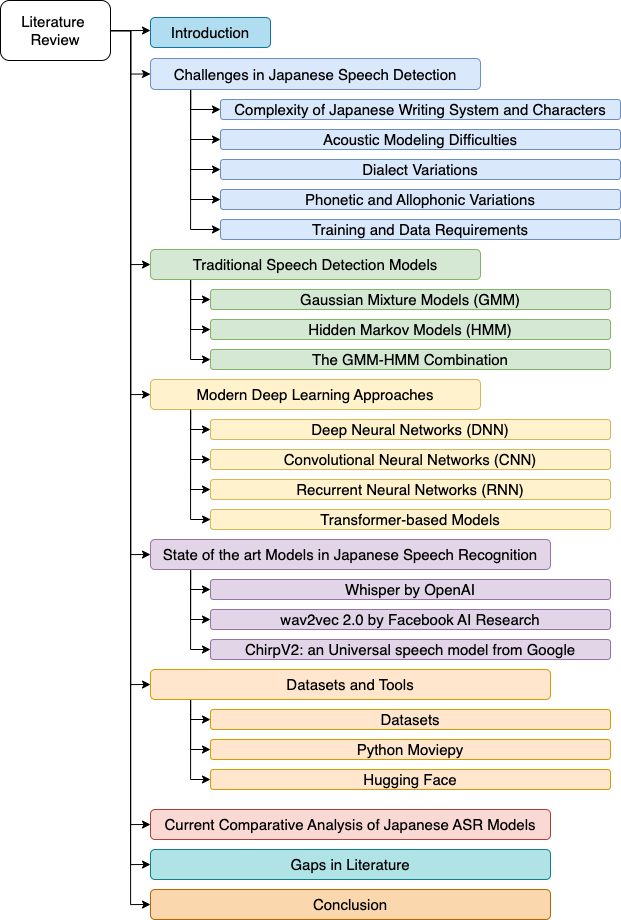
\includegraphics[width=.9\textwidth]{mainmatter//images/mindmap.png}
    \caption{Literature Review Mind Map}
\end{figure}

However, to apply these technologies to the Japanese language may pose few challenges due to its complex writing systems, phonetic ambiguities, and dialectal variations. In this chapter, the challenges of Japanese speech detection and the traditional and modern ASR models will be reviewed. The state-of-the-art model like Whisper, wav2vec, and Chirp will also be discussed based on their applicability to Japanese. By identifying the key challenges and gaps in existing research, this chapter prepared for a focused analysis of Japanese-specific ASR systems.

\section{Challenges in Japanese Speech Detection}
\subsection{Complexity of Japanese Writing System and Characters}
The complexity of Japanese writing system and character can cause challenge in ASR system especially in end-to-end neural network architectures. Japanese writing system is a combination of multiple character sets, such as the Hiragana, Katakana, Kanji (ideographic characters), Roman letters and various symbols, leading to a considerably larger and more varied character \parencite{rose2019unique}. As mentioned by \textcite{Ito2016End-to-end,ito2017}, the number of possible Japanese character labels can exceed several thousand.

A single character of kanji may have a few ways to pronounce it because each character of kanji has Onyomi (Chinese derived) and Kunyomi (native Japanese) readings, and these readings can change depending on the word context \parencite{curtin2020japanese}. Because of this ambiguity, the ASR system must be able to model and distinguish numerous acoustic differences in the speech data with same sound. The training model must be able to handle thousands of character and each of the character is potentially linked to multiple context dependent phonetic outcome which require a significant computational resources and large scale training data to ensure adequate coverage \parencite{Ito2016End-to-end,ito2017}.


% \subsection{Acoustic Modeling Difficulties}
% \textcite{ito2017} also discussed that one of the core acoustic modeling challenges in Japanese ASR is from the huge number of characters that must be predicted directly from the acoustic signal. This large number of characters can reach thousands of label and can quickly increase the number of parameters in the acoustic models. Because of this, a traditional model like HMM-GMM and more recent end-to-end framework to face challenges when scaling into these high quantity of label sets. The combination of different character sets like Kanji, Hiragana, Katakana, Roman letters, digit and symbol forces the acoustic model to handle a massive output data, which makes the straightforward end-to-end approaches less efficient\parencite{glasmachers17a}. 

% The intonation and pitch accent in Japanese language is important to distinguish between words with similar sound but has different meaning. However, to accurately modeling these patterns is challenging because it is not depends on the specific word that being spoken but also on the sentence structure and grammatical context \parencite{yasuda2022}. This is different from the languages where the pronunciation can often be predicted based on the nearby sound because Japanese language require a deeper understanding of the overall linguistic context to capture the correct pitch accent.



\subsection{Dialect Variations}  
Another notable challenge in Japanese speech detection is dialectical variation that exist in the language. These dialects usually different from the standardized Tokyo based variety that is referred to as standard Japanese \parencite{takahashi2024comparison}. As mentioned by \textcite{Imaizumi2020Dialect-Aware} that simply merging merging dialectal data with standard Japanese data into a single multi-condition training set often proves insufficient. The dialect specific pattern become saturated and leads to inefficient modelling and reduce the recognition accuracy. This issue can be addressed by integrating dialect labels as auxiliary features within the end-to-end ASR modeling framework. By explicitly encoding dialect information into the model, the recognition performance is improved by 19.2\% relative error reduction \parencite{Imaizumi2020Dialect-Aware}.

Another approach suggested by \textcite{imaizumi2022} is by employs a multi-task learning framework that able to optimize both dialect identification (DID) and multi-dialect ASR. This is achieveable by jointly training for dialect classification and ASR, the system exploits the strong interdependencies between acoustic-phonetic cues that is important for identification of dialectal features and linguistic structures that is crucial for accurate transcription. Three proposed architectures on how DID and ASR are integrated are as below:

\begin{enumerate}
    \item DID2ASR: First performs dialect identification, then uses the predicted dialect label to inform ASR decoding. 
    \item ASR2DID: Reverses the order, first performing ASR and then using the recognized text to identify the dialect. 
    \item DID+ASR: Conducts dialect and ASR prediction jointly, using distributions over dialect classes rather than a single predicted label.
\end{enumerate}

 
From these experiments demonstrate that multi-task learning with DID and ASR reduces word error rates and improves dialect classification accuracy \parencite{takahashi2024comparison}. 

% \subsection{Phonetic and Allophonic Variations}
% A study conducted by \textcite{Nguyen2002ModelingFA} highlighted the impact of modeling frequent allophones to enhance recognition accuracy in the Japanese ASR systems. They observed that Japanese's predominant Consonant-Vowel (CV) syllabic structure leads to a skewed frequency distribution of certain CV pairs (e.g., /n-o/, /sh-i/, /k-a/), with frequent allophonic variations often misclassified by standard ASR systems that rely on broad phonemic units. 

% Aside from Phonetic variation, another challenge in Japanese speech detection is that the Japanese allophonic variation. These variation is influenced by factors such as vowel length, nasalization and gemination that  often lead to context-dependent changes in phoneme realization. For traditional speech recognition, allophonic variation poses a certain challenges \parencite{halpern2008role}. However, for refined acoustic models that explicitly capture frequent allophones by isolating allophones associated with common CV combinations, these challenges can be mitigated. These models dedicate specific mixture densities and Gaussian components to high-frequency variants and allows the system to better differentiate subtle acoustic differences.

% \subsection{Training and Data Requirements}
% The quality of the Japanese speech detection system is relying heavily on the quality of the available training data as well as the methods and techniques employed during model training. As highlighted by \textcite{Karita2021} , Japanese ASR is often benchmarked using substantial corpora, such as the 581-hour Corpus of Spontaneous Japanese (CSJ). Similarly, \textcite{yasuda2022} mentioned that large-scale textual resources are essential for pre-training language models like PnG BERT that can capture both character and phoneme-level representations, enabling important aspect such as pitch-accent-aware TTS.

% It is important to do pre-training on a large text corpus as example shown by \textcite{yasuda2022} that uses massive raw text and phoneme transcriptions to build strong contextual representations. While it skips paired speech-text data during pre-training, fine-tuning on high-quality and labeled speech is still necessary to align phoneme and acoustic features effectively. Fine-tuning strategies, such as layer freezing and gradual unfreezing, also can can help adapt pre-trained text models like PnG BERT in the speech recognition tasks \parencite{ardestani2024study}. This ensures linguistic knowledge from pre-training is preserved while shifting focus to acoustic features, especially when speech datasets are smaller. 


\section{Traditional Speech Detection Models } 
\subsection{Gaussian Mixture Models (GMM)}
GMM have been the earliest technology used for developing Japanese speech detection and recognition systems because of their capability in capturing the statistical distribution of speech features very well \parencite{Imaishi2022Examination}. Because of the absence of word boundaries and the nuances of pitch accent in the Japanese language, it is really complicated to understand the context of the spoken words. However, GMM would be useful by employing probabilities to manage and characterize intricate patterns \parencite{sun2020subspace}. For example, \textcite{povey2011subspace} were able to use GMM to model phoneme-based acoustic features, and this approach led to a good performance of speech recognition systems.

 \textcite{Imaishi2022Examination} developed an approach within the EM algorithm that leads to the stabilization of the GMM parameters as well as increasing the discriminative power of the model in cases where there is not much evaluation data available. In other work, \textcite{povey2011subspace} point out that it is possible to represent the distribution of speech features in GMM mode by employing a combination of several Gaussian components. This way the GMM ca n account for the phonetic or speaker variability which is known to be present during word is being pronounce.

\textcite{Takami2020Performance} emphasized a different direction which starts with the creation of the Universal Background Model, which is a Gaussian Mixture Model calculated from the collection of a large number of speech samples from every dialect. To develop a model of the characteristics of a given UBM, the UBM is modified through Maximum A Posteriori (MAP) Adaptation. This method adjusts parameters of the UBM such as mean vectors, covariance matrices, and mixture weights depending on the individual’s data \parencite{dehak2009support}. Studies also  have shown that the use of speaker factor space constructed in the GMM and Joint Factor Analysis (JFA) can greatly improves the accuracy and efficiency of GMM systems \parencite{matrouf2011modeling}.

\subsection{Hidden Markov Models (HMM)}
HMM is working quite well with Japanese speech detection because of the incorporation of the acoustic and temporal characteristics of speech, including the difficulties found in the encoding of Japanese speech \parencite{Tokuda1999Application}. Moreover, HMM is so useful in ASR because they are very efficient in the representation of time varying systems by a succession of discrete time states. A unique segment of the speech signal is represented in each state, and the segment is described using a specific set of acoustic features \parencite{juang1991hidden}. ASR systems incorporated with HMM are more superior in portraying Japanese speech characteristics’ rhythm and tone including essential features like pitch accent and moraic timing which features will enhance the performance of the systems on the phonology aspects of the language \parencite{Tokuda2000HMM}.

ASR systems based on HMMs give quite satisfactory results especially on languages like Japanese because it is a possible to interpolate between a discrete set of states, where each state stands for a segment of the speech signal that has distinct acoustic features like pitch, duration, and phoneme quality \parencite{juang1991hidden}. To further Increase Japanese ASR project, few other models is used along with HMM which is context-sensitive such as Tri-phone method. Tri-phone method is a phonetic expansion that employs phonetics of the neighbor sounds to the phoneme as context in order to increase the recognition accuracy by taking into account the co-articulation that takes place during fast speech production \parencite{Tokuda2000HMM}. Other models by \textcite{gales2008application} were used together with HMM are Maximum Mutual Information and Minimum Phone Error which are useful for optimizing the parameters of the HMM and improve the recognition performance. 


\subsection{The GMM-HMM Combination}
The GMM-HMM model uses GMM for the observation probabilities corresponding to each state of the HMM. Each state of an HMM is assumed to have a library of Gaussian mixtures with which the state’s acoustic feature is pooled. Because transition probabilities of each state are determined by the HMM, temporal dependency of speech is well modelled. This combination allows the system to account for some of the variations in speech signals, such as those related to accent and the differences in the pronunciation of words in the Japanese language \parencite{taheri2006fuzzy}. While HMMs trained with large datasets under maximum likelihood criteria may have limited discriminative power, incorporating GMMs as observation models captures a broader range of acoustic variations. This method works really well for Japanese language, which are sensitive to the duration of phonemes in the context of the language.

Furthermore, the integration of GMM and HMM eliminates the need for applying state-of-the-art feature extraction techniques like Mel-Frequency Cepstral Coefficients (MFCC), hence increasing recognition performance \parencite{nicita1}. This hybrid approach has been successful in speaker-dependent as well as in speaker-independent systems. When fuzzy clustering and the expectation-maximisation algorithm are used, lower error rates are usually obtained by GMM-HMM than the methods used in isolation. For example, in a paper on speech data collected in a noisy environment, it was demonstrated that GMM-HMM provided much improvement in recognition performance over the conventional HMM scheme \parencite{taheri2006fuzzy, nicita1}.


\section{Modern Deep Learning Approaches}
\subsection{Deep Neural Networks (DNN)}
The use of DNN in conjunction with HMM, also known as DNN-HMM has been shown to improve performance in Japanese speech recognition tasks. \textcite{seki2014comparison} compared syllable-based and phoneme-based DNN-HMM and found that the syllable-based DNN-HMM was better, as its parameter space is less coupled with the context of the syllables. They reported that an 11\% relative decrease in the WER for triphone DNN-HMMs over syllable-based DNN-HMMs when used on large databases such as ASJ+JNAS. The multilayered structure of DNNs makes it much suitable for developing models of contextual dependencies for speech signals \parencite{hojo2018dnn}. GMM-HMM models are less effective compared to DNN when the task involves the estimation of posterior probabilities. In particular, pre-training with restricted Boltzmann machines has been quite useful for weight initialization, the vanishing gradient problem, and overall performance \parencite{Mimura2013CSJ}.

\textcite{mu2020japanese} developed a double-deep neural network for the evaluation of Japanese pronunciation to address the problems of text-to-speech alignment and scoring. The DDNN integrated CNN and RNNs with attention and it is effective for detecting pronunciation mistakes. \textcite{lin2017dnn} noted the importance of addressing the particular problem of the lack of annotated Japanese speech corpora by emphasizing the use of transfer learning with DNN. First, pre-training on large universal datasets increases the generalization ability. Then, fine-tuning on Japanese databases enhances the performance that is critical in low-resource applications. The authors were also able to use CNN and recurrent architectures to attend to the granularity features of the Japanese language.

\subsection{Convolutional Neural Networks (CNN)}
There is difficulties in the visual speech recognition areas and specifically within lipreading because a limitation for the use of CNNs for phoneme recognition tasks was considered to be the number of training datasets \parencite{noda2014lipreading}. The research was conducted using elastic net regression on a seven-layer CNN structure and 58\% of phoneme recognition accuracy was obtained for Japanese datasets. Building upon this work, \textcite{yalta2019cnn} constructed a functional speech recognition framework inclusive of several types of words spoken intended for tight spots like houses. There are more focused methods for connecting microphones such as incorporating residual connections and batch denormalization. 

\textcite{noda2014lipreading} investigated the use of CNNs for solving the problem of creating a Japanese speech acoustic model. CNN used to encode the frequency-time domain images and properly exploit the spatial and temporal aspects. The C-nets employed in this model aided in recognizing fine speech traits that improved performance in terms of recognition in contrast to the prevalent GMMs and HMMs methods. The combination of CNNs with attention mechanisms has yielded some results in the accurate detection of Japanese speech. This integration has been beneficial in increasing accuracy and interoperability during the detection of long utterances and multi-speaker datasets \parencite{Mukohara2015Emotion}.


\subsection{Recurrent Neural Networks (RNN)}
In the work of \textcite{takeuchi2020real}, a novel design of the RNN is introduced, which enables the processing of input speech while removing noise caused by the room impulse response. This network mitigates the vanishing and exploding gradient problems often seen in RNNs while also keeping the parameter count low, making it very suitable for real-time applications. \textcite{Kida2016LSTM} investigated linear prediction filters based on LSTM. Their method trained an LSTM which did not require direct access to raw information and thus can extract features from distorted signals, as an LSTM estimated linear prediction coefficients. 

\textcite{Kubo2014DeepLearning} broadened approaches incorporating RNNs into synthesizing speech for Japanese, particularly focusing on improving prosody and intonation. Their work underscored the necessity to consider the sequential modelling features of RNNs units, especially LSTMs, techniques for natural voice synthesis of Japanese language sounds. \textcite{takeuchi2020real} took advantage of the RNN-based architectures for the acoustic modelling for Japanese ASR. They showed that even though GRUs have a simpler gating strategy than LSTMs, they could achieve a similar level of classification accuracy with lower compute requirements. Then, the studies on bidirectional LSTMs (BLSTMs). \textcite{imaizumi2022} revealed that they could utilise the past context and the future context of the signal for better performance of the speech recognition device. Many applications of automatic speech recognition in which the Japanese language is used have demonstrated that BLSTMs are particularly helpful for modelling complex phonological and prosodic structures of the Japanese language.


\subsection{Transformer-based Models}  
\textcite{taniguchi2022transformer} propose a series of Transformer-based ASR models aimed at improving Japanese speech recognition, particularly in the context of simultaneous interpretation. They investigate the possibility of utilizing auxiliary input like the source language text to resolve issues such as disfluencies, hesitations, and self-repairs commonly observed in the interpreter speech which helps to improve the transcription quality \parencite{Futami2020Bidirectional}. The models combined audio and text data via multi-modal transformer encoders and decoders, which offers a broader scope of recognition by using previously provided source language text for interpreter training programs \parencite{taniguchi2022transformer}.

A wide range of datasets for source text and simultaneous interpretation speech are however not readily available, so the authors use a adapted speech translation corpora from MuST-C and CoVoST 2 while also introducing TED based Japanese texts for evaluation purposes \parencite{taniguchi2022transformer}. With an additional goal of enhancing performance, the authors fine-tune the source language text encoder by using large machine translation corpora which helps in lowering the word error rates during translation of English, Dutch, German and Japanese \parencite{Taniguchi2024Pretraining}. Results consistently demonstrate that incorporating source language text into Transformer-based ASR models significantly improves recognition performance, with the greatest impact observed when auxiliary input is introduced at later stages of the audio encoding and decoding process \parencite{Futami2020Bidirectional}.

\section{State of the art Models in Japanese Speech Recognition}
\subsection{Whisper by OpenAI}
Large scale weak supervision has emerged as one of the major approaches in speech recognition as noted by \textcite{radford2023robust} in their development of whisper model that has been trained on multilingual and multitask audio datasets that has a combined duration of 680,000 hours. This work is a continuation to the self-supervised methods such as Wav2Vec 2.0 \parencite{baevski2020wav2vec}, which demonstrated learning without supervision from audio without any human-provided labels. However, dataset-specific fine-tuning is often necessary to obtain good performance, whereas with Whisper such reliance is reduced because of the efficacy of weak supervision. 

By scaling weak supervision across diverse datasets, Whisper able to bypass the need for dataset-specific adaptation while able offer a robust zero-shot performance across languages and tasks. The authors also mentioned that by using this method, it will ensure the generalization and the robustness of the model while at the same time addressing main limitation in traditional models that is struggled to transcribe unfamiliar audio. This method also resulting in the models to have similar trends with other state of the art model in machine learning where a large, diverse datasets will improve model resilience which is align the with the advancements in computer vision \parencite{kolesnikov2020big} and NLP \parencite{radford2019language}.The Whisper model’s architecture, a simple encoder-decoder Transformer, reinforces the effectiveness of minimal preprocessing and sequence-to-sequence training, simplifying the transcription pipeline while achieving near-human-level accuracy.

\begin{figure}[!ht]
    \centering
    
\includegraphics[width=.9\textwidth]{mainmatter//images/image.png}
    \caption{Whisper WER cited from \cite{radford2023robust}}
\end{figure}

Based on the work of \textcite{radford2023robust}, there is further research that seeks to improve the performance of multilingual models on tasks that involve a japanese language. \textcite{bajo2024efficient} detail their work on adapting OpenAI’s Whisper model to enhance its performance in ASR for the Japanese language. The research draws attention to the dilemma faced in balancing the multilingual being and the accuracy of an English-only product, ReazonSpeech, that seeks to maximize on the Japanese language ASR, which is monolingual in nature. By using a Japanese dataset while utilizing Low-Rank Adaptation (LoRA) and fine-tuning methods, they were able to lower Whisper-Tiny’s Cumulative Expenditure Rate (CER) from 32.7\% to 14.7\%. This fine tuning method showed that smaller multilingual models give more promising result, after being tuned for the desired language outperform their larger baseline models, for example the case of the Whisper-Base model \parencite{bajo2024efficient}.


\begin{table}[ht]
    \centering
    \caption{WER and CER performance of Whisper models. Reproduced from \cite{bajo2024efficient}.}
    \begin{tabular}{p{4cm}|p{3cm}|p{3cm}}
    \hline
    \textbf{Model}        & \textbf{WER (\%)} & \textbf{CER (\%)} \\ \hline
    Whisper Tiny          & 47.48             & 32.74             \\ 
    Whisper Base          & 29.81             & 20.20             \\ 
    Whisper Small         & 16.14             & 9.89              \\ 
    Whisper Medium        & 10.84             & 6.86              \\ 
    Whisper Large         & 7.41              & 4.77              \\ \hline
    Whisper Tiny + LoRA   & 33.16             & 20.83             \\ 
    Whisper Base + LoRA   & 23.36             & 14.50             \\ 
    Whisper Small + LoRA  & 14.90             & 9.16              \\ \hline


    \end{tabular}
    \label{tab:whisper-performance}
    \end{table}
    
  
\subsection{wav2vec 2.0 by Facebook AI Research}
The research conducted by \textcite{baevski2020wav2vec} proved that self-supervised learning greatly reduces the dependency on large amounts of labeled data in speech recognition. They achieved this by using a technique called wav2vec 2.0. With this method, models are trained over a significant set of unlabeled speech data by masking the raw audio inputs and then treating a contrastive task. Thereafter, a model can be fine tuned using a limited set of labeled data which enables it to perform better when compared to semi-supervised techniques. Furthermore, according to \textcite{baevski2020wav2vec}, while their approach performed well with all the available labeled data by raising the WER to 1.8\% for clean data and 3.3\% for other data, it went even better with 10 mins of labeled and 53k hours of unlabeled data which had WER rates of 4.8\% and 8.2\%.
\begin{table}[h!]
    \centering
    \caption{WER on Librispeech dev/test sets using 10 minutes of labeled data and different unlabeled data setups.}
    \begin{tabular}{@{}lcccc@{}}
    \toprule
    \textbf{Model}      & \textbf{Unlabeled Data} & \textbf{LM} & \textbf{dev (clean)} & \textbf{test (other)} \\ \midrule
    Discrete BERT  & LS-960                 & 4-gram  & 15.7           & 25.2           \\
    BASE                                     & LS-960                 & 4-gram+Transf. & 8.9            & 15.6           \\
                                             &                        & Transf.        & 6.6            & 12.9           \\
    LARGE                                    & LS-960                 & Transf.        & 5.0            & 10.0           \\
                                             & LV-60k                 & Transf.        & \textbf{4.6}   & \textbf{8.2}   \\ \midrule
    \textbf{Highlighted Result}     & LV-60k (53k hours)     & Transf.        & \textbf{4.8}   & \textbf{8.2}   \\ \bottomrule
    \end{tabular}
    \end{table}

In Japanese speech recognition, self-supervised learning (SSL) has emerged as one of the major tools for tackling the problems of dialectal diversity and low-resourced datasets. \textcite{miwa2023dialect} showcased what they refer to as successful adaptation of the wav2vec 2.0-based XLSR model to the Corpus of Japanese Dialects (COJADS), a collection of data capturing various dialects from different regions of Japan. They reported significant gains in ASR metrics for dialectal speech, achieving CER reductions of as much as 8.9\% relatively to the models only trained on tagged data. 


\subsection{ChirpV2: an Universal speech model from Google}
\textcite{zhang2023google} demonstrated a novel technique that scales ASR to more than a hundred languages, this is achieved with the aid of large multilingual datasets with self-supervised learning, they refer to their model as the Universal speech model. The model was pretrained on 12 million hours of unlabelled audio data collection of 300 languages, in addition to 90 thousand hours of multilingual labelled audio data. One of the crucial innovations is BEST-RQ (BERT-based Speech pretraining with Random-projection Quantizer) because it improves the performance of speech representation without complicated quantization modules. 

The model also outperformed specialized models including Whisper that have previously been trained with more data. In addition to this, chunk-wise attention is used to solve the performance drop-off problem that USM has with long audio, allowing USM to transcribe long audio. Other language resource enabling techniques such as noisy student training and adapter modules have enhanced USM performance with low resource and unseen languages considerably, as it did with low resource languages ensuring a robust ASR system \parencite{zhang2023google}. USM proves the efficacy of self-supervised models in minimizing multilingualism and far supersedes existing standards for ASR systems.
\begin{table}[H]
    \centering
    \caption{Word Error Rate (WER) Comparison of ASR Models}
    \begin{tabular}{|l|c|c|c|}
    \hline
    \textbf{Dataset}        & \textbf{USM-CTC (\%)} & \textbf{USM-LAS (\%)} & \textbf{Whisper (\%)} \\ \hline
    YouTube (en-US)         & 13.7                  & 14.4                  & 17.7                 \\ \hline
    YouTube (CORAAL)        & 18.7                  & 19.0                  & 27.8                 \\ \hline
    SpeechStew (en-US)      & 26.7                  & 29.8                  & -                    \\ \hline
    FLEURS (62 languages)   & 12.1                  & 11.2                  & 13.2                 \\ \hline
    Multilingual (YouTube)  & 15.5                  & 12.5                  & 23.9                 \\ \hline
    \end{tabular}
    \label{tab:wer_comparison}
    \end{table}

\section{Current Comparative Analysis of Japanese ASR Models}
A comparative analysis that carried out by \textcite{Karita2021} shows that Conformer-based models perform better than Conformer BLSTM architectures, as they obtained 4.1, 3.2, and 3.5 character error rates for CSJ in eval1, eval2, and eval3 tasks respectively. It is noted that both the BLSTM and Conformer models have character error rates below 7\% and the character error rate is lower when using Conformer Itself. Conformer encoders also offer increased accuracy and efficiency, with a throughput of 628.4 utterances processed per second and 430.0 for the BLSTM models. The scope of the work also emphasizes the importance of the analysis of the specific problem of training parameters optimization, noting the importance of the implementation of SpecAugment, exponential moving average (EMA) and variational noise (VN). The SpecAugment technique results in the largest shifts which affect the performance. The integration of the Conformer transducers with the described set of training approaches surpasses all existing solutions in Japanese ASR and open the path for further development \parencite{Karita2021}.

\begin{table}[h!]
    \centering
    \caption{Character error rates on CSJ dev/eval1/eval2/eval3 sets cited from \cite{Karita2021}.}
    \begin{tabular}{l|l|c|c|c}
    \hline
    \textbf{Encoder}   & \textbf{Decoder}   & \textbf{Param} & \textbf{Utt/sec} & \textbf{CER [\%]} \\ \hline
    BLSTM              & CTC               & 258M             & 430.0            & 3.9 / 5.2 / 3.7 / 4.0 \\ 
    BLSTM              & attention         & 309M             & 365.5            & 3.8 / 5.3 / 3.7 / 3.7 \\ 
    BLSTM              & transducer        & 274M             & 297.6            & 3.8 / 5.1 / 3.7 / 4.0 \\ 
    Conformer          & CTC               & 117M             & \textbf{628.4}   & 3.1 / 4.1 / 3.2 / 3.5 \\ 
    Conformer          & attention         & 124M             & 534.8            & 3.3 / 4.5 / 3.3 / 3.5 \\ 
    Conformer          & transducer        & 120M             & 376.1            & \textbf{3.1 / 4.1 / 3.2 / 3.5} \\ \hline
    \end{tabular}
    \label{tab:cer_comparison}
    \end{table}

Another comparative analysis in the domain of the Japanese language is presented by \textcite{takahashi2024comparison}, focusing on the accuracy of speech recognition for different dialects. The study evaluates three models: Whisper, XLSR, and XLS-R, which are self-supervised learning frameworks. The Whisper model significantly underperformed for any Japanese outside of standard Japanese, recording a 4.1\% CER only after it has gone through fine tuning. However, when the accuracy is low when the language identification marker is absent where some instances of being higher than 100\%.This marks the weakness of Whisper in terms of its application for wide ranging applications in different dialects of Japanese. However, Whisperer and XLS-R both of which were trained on multilingual speech data show improvement in the recognition of Japanese dialects. These models apply multi-task learning paradigms such as DID and ASR to increase their efficiency. Multi tasking adds significantly to the dialect accuracy and a three-step efficient training of the models reduce the CER by 3-4\% relative to conventional transfer learning. Some dialects, especially those from Kyushu and Chubu, have larger CER than those spoken in Kanto, where there is a greater linguistic affinity \parencite{takahashi2024comparison}.

Current comparative analysis from these studies shows that several challenges need to be addressed. A study to compare the state of the art models in Japanese ASR is needed because from previously mentioned paper it is clear that the performance of the models varies depending on the dataset and the task. The Whisper model is the most accurate in the Japanese language, but it is not as effective in dialectal speech. The XLSR and XLS-R models are more effective in dialectal speech, but they are not as accurate as the Whisper model in standard Japanese. The Conformer model is the most accurate in standard Japanese, but it is not as effective in dialectal speech\parencite{takahashi2024comparison}. The study will provide a comprehensive comparison of the state of the art models in Japanese ASR, which will help to identify the strengths and weaknesses of each model and to determine which model is the most effective for a given dataset and task.

\begin{table}[H]
    \centering
    \caption{Comparison of ASR accuracy on two datasets, Standard Japanese (CSJ) and Japanese dialects (COJADS) cited from \cite{takahashi2024comparison}.}
    \begin{tabular}{c|c|c|c}
    % \begin{tabular}{p{2.7cm}|c|p{2cm}|p{2cm}}

    \hline
    \textbf{Pre-Trained Model Name} & \textbf{Adaptation Method} & \textbf{CER [\%] CSJ} & \textbf{CER [\%] COJADS} \\ \hline
    Whisper-medium (zeroshot)       & -                              & 25.6*                 & 116.0*                   \\ \hline
    Whisper-medium                  & full finetuning                & \textbf{4.1}          & 32.9                     \\ \hline
    XLSR                            & full finetuning                & 6.5                   & 34.1                     \\ \hline
    XLSR                            & 3-steps finetuning             & -                     & 30.0                     \\ \hline
    XLS-R                           & full finetuning                & 6.1                   & 32.6                     \\ \hline
    XLS-R                           & 3-steps finetuning             & -                     & \textbf{29.2}            \\ \hline
    \multicolumn{4}{l}{\footnotesize *After post-processing with kanji-to-kana conversion.} \\
    \end{tabular}
    \label{tab:asr_comparison}
\end{table}

\section{ Dataset and Tools }
\subsection{Datasets}
The dataset used in the Japanese ASR system is crucial for the performance of the model. The TED talks dataset is one of the most widely used datasets for Japanese ASR research \parencite{Afouras}. This dataset contains speech data from TED talks in multiple languages, including Japanese. The TED talks dataset is useful for evaluating the performance of ASR systems on real-world speech data and for comparing the performance of different models.

Another dataset that is commonly used in Japanese ASR research is the Corpus of Spontaneous Japanese (CSJ). It contains 581 hours of spontaneous speech data, which is divided into training, development, and evaluation sets \parencite{Andos}. The CSJ dataset is annotated with phonetic, prosodic, and morphological information, making it a valuable resource for training and evaluating ASR systems. 

For dataset that contain dialectical speech, the Corpus of Japanese Dialects (COJADS) is a valuable dataset that contains speech data from various Japanese dialects. It is especially useful for training ASR systems to recognize and transcribe different dialectical nuances, thereby enhancing system robustness in diverse linguistic contexts \parencite{kibe2018intonational}.

\subsection{Python Moviepy}
MoviePy is a Python library for video editing that can be used to extract audio from video files. It provides a simple and intuitive interface for working with video and audio files, making it easy to extract audio clips from video files \parencite{boishakhi2021multi}. One of the key features to use MoviePy in this study is to extract audio from video files and convert them into a format that can be used for training ASR models.

\subsection{Hugging Face}
Hugging Face is a platform that provides a wide range of pre-trained models for natural language processing tasks, including speech recognition. It offers a variety of models that can be fine-tuned on custom datasets to improve performance on specific tasks \parencite{boishakhi2021multi}. In this study, Hugging Face will be used to access pre-trained models for Japanese ASR. These model will be downloaded from Hugging Face and analyze the performance of the models based on the dataset used in this study.

\section{Gaps in Literature}
Based on the literature review, shows that there is several gaps in the research on Japanese ASR. One of the area is the insufficient exploration of how state-of-the-art models can be adapted to the specific nuances of the Japanese language. Although there is few study that evaluate the performance of these model, but there is no notable research that focusing on evaluating the state of the art models in Japanese ASR. Another research gap from the literature review is the lack of focus on the performance of these models when dealing with dialectical variations of Japanese. Although research has been conducted on their effectiveness with standard Japanese, there is a clear need for further work on how these newly developed models perform when handling dialectical speech. Lastly, another gap identified is the underexplored area of these models application in real-time environments. Despite some investigations into their use in real-time scenarios, additional research is required to optimize these models for applications where quick response times are essential.

\section{Conclusion}
This chapter highlighted the challenges in Japanese ASR system that is its writing systems, phonetic variations, and dialectal diversity. The evolution of traditional ASR model to the cutting-edge technologies also has been highlighted in this chapter. Despite the advancements of the model and ASR framework, there is still a gap in adapting these models to Japanese-specific contexts, especially in handling informal speech and dialects. There is still work to be done to further refine the accuracy, speed, and dataset availability to advance Japanese ASR. This result can be used as a foundation for developing more effective and inclusive speech-to-text solutions tailored for Japanese language. For the dataset and tools, TED talks, CSJ, and COJADS are the most commonly used datasets for Japanese ASR research. To extract audio from video files, Python Moviepy is used and to access pre-trained models for Japanese ASR, the model will be obtain from Hugging Face. 